\documentclass{book}
\usepackage{myHead}
\graphicspath{
	  {images00-01/}{images00-02/}
		  {images01-01/}{images01-02/}{images01-03/}
		}
\usepackage{showlabels}
% будет показывать ссылки прямо в pdf. когда файл готов, лучше убрать
\usepackage{booktabs}

\renewcommand{\descriptionlabel}[1]{\hspace{\labelsep}\textsc{#1}}

\newcommand{\Prob}{\mathsf P}
\newcommand{\D}{\mathsf D}
\newcommand{\M}{\mathsf M}

\newenvironment{solution}
{
	\vspace{0.5em}

	\noindent\textsc{Решение.}
}
{
	\par\hfill\square
}
\renewcommand{\qedsymbol}{$\blacksquare$}



\begin{document}
\title{Теория вероятностей -- 1}
\maketitle
\tableofcontents

\section*{Некоторые обозначения}
\label{sec:tos}
\begin{enumerate}
  \item Символ $ \sum_{i=1}^n A_i = A $, применённый к множествам $ A_i $,
    означает объединение \textsl{непересекающихся} множеств, то есть, что $ A =
    \bigcup_{i=1}^n A_i $, причём для любых $ k $, $ l $ выполняется $ A_k \cap
    A_l = \varnothing$.
  \item Символ $ A_i\uparrow A $ означает бесконечное объединение возрастающей
    последовательности множеств, то есть, что $ \bigcup\limits_{i=1}^\infty A_i
    = A$, причём для любого $ k $ выполняется $ A_k \subseteq A_{k+1} $.
\end{enumerate}


\part{Дискретный случай}
\chapter{Элементарная теория вероятностей}
\section{Вероятностная модель эксперимента с конечным числом исходов}
Пусть проводится некий эксперимент с \emph{конечным} количеством исходов,
которые мы обозначим через $ \omega_1, \dots, \omega_N $.

Эти исходы будем также называть \emph{элементарными событиями}, а их
совокупность  
\[
	\Omega = \{ \omega_1, \dots , \omega_N\}
\]
(конечным) \emph{пространством элементарных событий} или \emph{пространством
исходов}.
Нахождение $ \Omega $ есть первый шаг в построении \emph{вероятностной модели}.
\begin{example} 
	Однократное подбрасывание монетки даёт, очевидно, $ \Omega = \{\text{Г}, \text{Р}\} $.
	Пространство элементарных событий для эксперимента с подбрасыванием монетки
	$n$ раз будет состоять из $ N(\Omega) = 2^n$ событий, каждое из которых будет определяться
наборами из $n$ значений типа Г или Р:
\[
	\omega_i = (a_1, a_2, \dots , a_n), \quad \text{где } a_i = \{ \text{Г},
	\text{Р} \}.
\]
В данном случае можно провести биекцию между событиями и подмножествами множества из $ n $
элементов, если считать, что Г обозначает взятые в это подмножество элементы, а
Р --- не взятые.
\end{example}

В примере выше мы считали \emph{упорядоченные} различно комбинации различными.
Чтобы отличить набор, не уважающий порядок, вводится обозначение $
[a_1,\ldots,a_n] $.

Рассмотрим такой случай на примере изъятия шаров с последующим
\emph{возвращением}.
\begin{example}
	Будем считать, что количество шаров $ M $, а длина комбинации $ n $. Общее количество таких
	комбинаций будет равно $ N(\Omega) = M^n $. Ни выше, ни здесь мы данный вывод
	никак не обоснуем, однако это легко сделать, воспользовавшись начальными
	знаниями комбинаторики и индукцией.

	Рассмотрим случай, когда порядок внутри комбинации не объявляется. Очевидно,
	различных комбинаций $ N(\Omega) $ тогда будет меньше. Покажем, что для этого
	случая  
	\[
		N(\Omega) = C^n_{M+n-1},
	\]
	где $ C^l_k := k!/(l!(k-l)!) $ --- <<число сочетаний из $ k $ элементов по $ l
	$>>. Доказательство будем проводить через индукцию по $ n $. Примем за $ N(M,
n) $ интересующее нас число, то есть количество возможных комбинаций длины $n$
из $ M $
шаров. 

	Простейшему случаю $ n = 1 $ соответствует простейшее заключение $ N(M, 1) = M
	$, что подтверждает нашу гипотезу. Заметим ещё, что $ N(k, 1) = k $ и для
	любого $ k \leqslant M $.

	Будем считать, что утверждение доказано для $ n $ и докажем его для $ n + 1 $.
	Поскольку порядок отсутствует, будем считать, что элементы расположены, к
	примеру, по неубыванию. В общем случае выберем некоторый эталонный порядок и
	пронумеруем шары: $ a_1, a_2, \dots, a_M $. В случае с $ N(M, n+1) $, легко заметить, что
	рассматривая отдельно все комбинации, в которых первыми элементами будут $ a_1
	$, $a_2$ и так далее, мы будем получать соответственно количество возможных
	комбинаций $ N(M, n)$, $N(M-1, n)$, $ N(M-2, n) $ и так далее. При этом просуммировав все
	эти числа, мы, конечно, получим интересующее $ N(M,n+1) $. А сделать это
	легко, поскольку все числа до $N(M, n)$ включительно, благодаря индукции, нам
	уже известны.

	Таким образом, осталось лишь доказать важную и для дальнейшего изучения
	формулу биномиальных коэффициентов
	\begin{equation}
		\label{eq:bin_coef}
		C^{l-1}_k + C^l_k = C^l_{k+1},
	\end{equation}
на чём мы останавливаться не будем. Скажем лишь, что это свойство лежит в основе
составления \emph{треугольника Паскаля}. Кроме того,  его легко доказать, заметив,
что первое слагаемое есть число комбинаций без порядка, в которые не входит
некий шар $ a_0 $, а второе --- общее число комбинаций длиной $ k $. Эту формулу
можно также вывести в лоб. 

Действительно, воспользуемся формулой \eqref{eq:bin_coef} и получим \qed
%TODO: proof
\end{example}

Тот же факт можно доказать проще. Пусть есть одна из таких комбинаций (без
порядка, но с повторениями) длины $ n $ с $ m $ возможными категориями шаров.
Тогда её можно представить как набор из $ n + m - 1$ единиц и нулей,
где, скажем, единица разделяет категории шаров. Поскольку категорий $ m $, то
разделителей будет $ m-1 $, а самих шаров по-прежнему $ n $. В такой комбинации
уже важен порядок, но в ней есть и повторения. Теперь к тому же исходных
множеств два. Выберем вместо этого тогда не сами элементы, а места под них.
Будем ставить в соответствие некоторым из $ m+n-1 $ мест $ m - 1 $
разделителей-единиц. При этом места не могут повторяться, а порядок вновь не
важен. Получили инъекцию из $ m-1 $ разделителей в $ m+n-1 $ мест. Согласно
одному из свойств биномиальных коэффициентов,  
\[
	C^{m-1}_{m+n-1} = C^{(m+n-1)-(m-1)}_{m+n-1} = C^n_{m+n-1}
\]
Действительно, мы выбирали $ m-1 $ единиц, хотя могли выбирать $ n $ нулей.
\qed



Перечислим ещё некоторые \textbf{свойства биномиальных коэффициентов}:
% TODO: свойства биномиальных коэффициентов

\begin{figure}[h!]
	\centering
	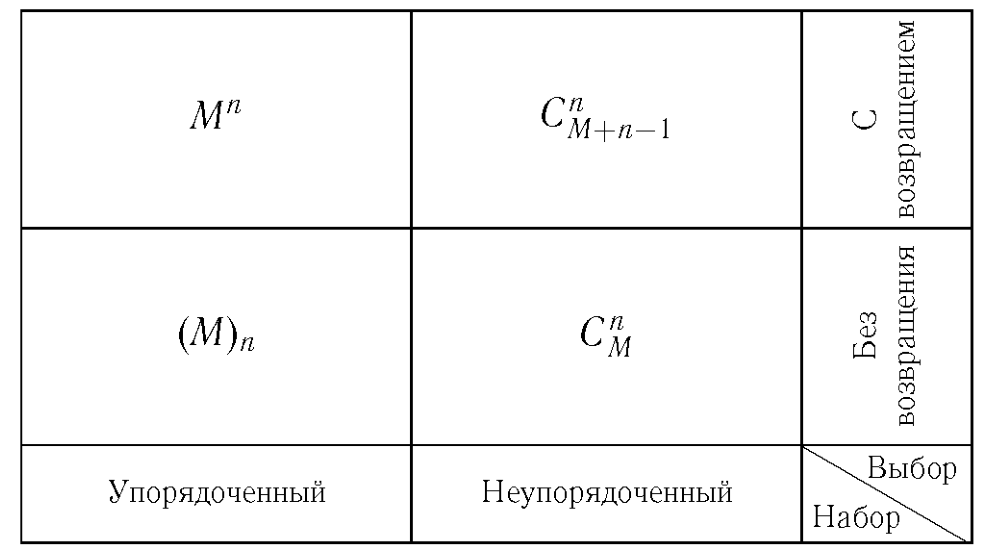
\includegraphics[width=0.8\textwidth]{Figures/table-1.png}
	\caption{Резюме}
	\label{fig:table-1}
\end{figure}


\subsection{Перестановки}
Перестановки без повторений $ n $ элементов осуществляются $ n! $ способами, это
легко проверить по индукции. 


\subsection{Ячейки и дробинки}
Выберем \emph{ячейки для дробинок}.
Пусть дробинки различимы. Тогда опыт описывается набором $ (a_1, \ldots, a_n) $.
Иначе --- набором $ [a_1, \ldots, a_n] $. Аналогично можно провести аналогию для
размещений с запретом (одна ячейка содержит не более одной дробинки) и без. В
первом случае имеем выбор с возвращением, во втором --- без. Имеем 
\begin{figure}[h!]
\begin{center}
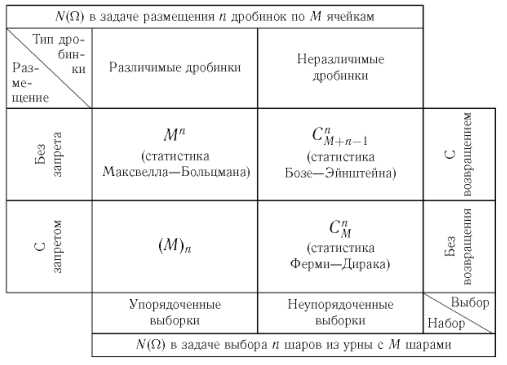
\includegraphics[width= \textwidth]{Figures/drob.png}
\end{center}
\label{fig:drob}
\end{figure}


\subsection{Событие}
\begin{definition}
	\emph{Событием} называем такое подмножество $ A \subset \Omega$ всех исходов,
	для которого по условиям эксперимента возможен однозначный ответ $ \omega \in
	A$ или $ \omega \notin A $. Событие $ \varnothing $ называем
	\emph{невозможным}, а $ \Omega $ --- достоверным.
\end{definition}

Объединение множеств $ A \cup B $ в том случае, когда они не пересекаются,
называется \emph{суммой} множеств и обозначается $ A + B $.

Система событий может образовать \emph{алгебру} $ \mathscr A $ с операциями $ \cup $, $ \cap $
и $ \setminus $, при условии $ \Omega \in \mathscr A $. Обычно берётся алгебра
всех подмножеств $ \Omega $.

\subsection{Вероятность}
Припишем каждому элементарному событию $ \omega_i \in \Omega $ некоторую
\emph{вероятность исхода},
обозначаемую $ p(\omega_i) = p_i $. Потребуем для этой величины выполнение
следующих условий: 
\begin{enumerate}
	\item $ 0 \leqslant p_i $,
	\item $\sum_{i=1}^N p_i = 1$ (\emph{нормированность}).
\end{enumerate}
Вероятность события тогда определим формулой 
\[
\mathsf P(A) = \sum_{\{i\colon\omega_i\in A\}} p_i.
\]
Перечислим некоторые \textbf{свойства вероятностей}: 
\begin{gather*}
		\mathsf P (\varnothing) = 0,\\
		\mathsf P (\Omega) = 1,\\
		\mathsf P (A \cup B) = \mathsf P(A) + \mathsf P(B) - \mathsf (A\cap B).
\end{gather*}


\begin{definition}
	Совокупность $ (\Omega, \mathsrc A, \mathsf P) $ называют \emph{вероятностным
	пространством}. Оно определяет \emph{вероятностною модель} эксперимента с
	конечным пространством исходов $ \Omega $ и алгеброй событий $ \mathsrc A $. 
\end{definition}



\section{Некоторые классические модели и распределения}
%TODO: section



\section{Условная вероятность}
%TODO: section



\section{Случайные процессы и их характеристики}
Заботят часто не столько элементарные события целиком, сколько лишь некоторые
числовые характеристики, зависящие от них (например, число решек в орлянке).

\begin{definition}
Всякая функция $ \xi(\omega) \in \mathbb R $, определённая на (конечном) $ \Omega $, будет
называться (простой) \emph{случайной величиной}.
\end{definition}

Обозначим (конечное) множество значений случайной величины $ \xi $ как $ X $, а
алгебру его подмножеств как $ \mathscr X $. Подмножество $ B \in \mathscr X $
можно интерпретировать как некоторое событие. Тогда	 
\[
	P_\xi (B) := \mathsf P\{\omega \colon \xi(\omega) \in B\}, \quad B \in \mathscr
	X. 
\]
\sloppy При этом ясно, что достаточно определить 
\[
	P_\xi(x_i) := \mathsf P \{\omega \colon \xi(\omega) = x_i\}, \quad x_i \in X
\]
вероятности прообраза каждого возможного значения.
Набор чисел $ \{ P_\xi(x_1), \ldots, P_\xi(x_m)\} $ называется
\emph{распределением вероятностей случайной величины $ \xi $}.

\begin{example}
	Случайная величина $ \xi $, принимающая значение 1 с вероятностью <<успеха>> и
	0 с вероятностью <<неуспеха>> называется \emph{бернуллиевской}. Для неё 
	\[
		P_\xi(x) = p^xq^{1-x}, \quad x=0,1.
	\]
	\emph{Биномиальной случайной величиной $ \xi $} называется случайная величина с вероятностями 
	\[
		P_\xi(x) = C^x_np^xq^{n-x}, \quad x = 0, 1, \ldots, n.
	\]
\end{example}

\begin{definition}
	Функция  
	\[
		F_\xi(x)=\mathsf P\{\omega\colon\xi(\omega)\leqslant x\}
	\]
	называется \emph{функцией распределения случайной величины $ \xi $}.
\end{definition}

Ясно, что 
\[
	F_\xi(x) = \sum_{\{i\colon x_i \leqslant x\}} P_\xi(x_i)
\]
и 
\[
		P_\xi(x_i) = F_\xi(x_i) - F_\xi(x_i-).
\]

Из определения вытекают следующие \textbf{свойства функции распределения}:
\begin{enumerate}
	\item $ F_\xi(-\infty) = 0 $, $ F_\xi(\infty) = 1 $;
	\item $ F_\xi(x+)=F_\xi(x) $.
\end{enumerate}

Иногда приходится рассматривать \emph{случайный вектор} $ \xi = (\xi_1, \ldots,
\xi_r)$, компоненты которого есть случайные величины. Например, в
мультиномиальном распределении. В этом случае набор вероятностей 
\[
		P_\xi(x_1, \ldots, x_r) = \mathsf P\{\omega\colon \xi_1(\omega) = x_1,
		\ldots, \xi_r(\omega)=x_r\},
\]
где $ x_i \in X_i $ --- области допустимых значений $ \xi_i $, называется
\emph{распределением вероятностей случайного вектора $ \xi $}, а функция 
\[
		F_\xi(x_1, \ldots, x_r) = \mathsf P\{\omega\colon \xi_1(\omega)\leqslant
		x_1, \ldots, \xi_r(\omega) \leqslant x_r\},
\]
$ x_i \in \mathbb R $, называется \emph{функцией распределения случайного
вектора $ \xi = (\xi_1, \ldots, \xi_r) $}.

Случайные величины $ \xi_1, \lsots, \xi_r $ называются \emph{независимыми}, если
для любых $ x_1\ldots,x_r\in X$ 
\[
	\mathsf P \{\xi_1 = x_1, \ldots, \xi_r = x_r\} = \mathsf
	P\{\xi_1=x_1\}\ldots\mathsf\{\xi_r=x_r\},
\]
или, что эквивалентно, для любых $ B_1,\ldots,B_r \in \mathscr X $ 
\[
	\mathsf P\{\xi_1\in B_1, \ldots, \xi_r\in B_r\} = \mathsf P\{\xi_1 \in
	B_1\}\ldots\mathsf P\{\xi_r\in B_r\}.
\]
Простейший пример независимых случайных величин можно получить, 
рассматривая схему Бернулли.

Важную роль играют функции от случайных величин, которые сами, конечно, являются
случайными величинами. Например, для $ \zeta := \eta
+ \xi$, $ z\in \mathbb R $ имеем  
\[
	P_\zeta(z) = \mathsf P\{\zeta = z\} = \mathsf P\{\xi +\eta = z\} =
	\sum_{\{(i,j)\colon x_i + y_j = z\}} \mathsf P\{\xi = x_i, \eta= y_j\}.
\]
Особенно важен случай независимых случайных величин $ \xi $ и $ \eta $. Там
\[
	\mathsf P\{\xi = x_i, \eta = y_i\} = \mathsf P\{\xi = x_i\} \mathsf
	P\{\eta=y_j\},
\]
и, значит,  
\[
	P_\zeta(z) = \sum_{\{(i,j)\colon x_i + y_j = z\}} P_\xi(x_i)P_\eta(y_j) =
	\sum_{i=1}^k P_\xi(x_i) P_\eta(z-x_i).
\]


\subsection{Характеристики случайных величин}
Сформулируем важнейшее понятие \emph{математического ожидания} случайных
величин. Обозначим $ p_i := \mathsf P\{\xi = x_i\} $. Интуитивно мы хотели
бы\footnote{Это предположение в дальнейшем получит в некотором смысле
подтверждение},
чтобы при наблюдении за значениями случайной величины $ \xi $ в <<$ n $
повторных независимых экспериментах>> при больших $ n $ значение $ x_i $
встретилось бы
примерно $ np_i $ раз. Тогда средним значением случайной величины будет равно
примерно 
\[
	\frac{1}{n} [np_1x_1 + \ldots + np_kx_k] = \sum_{i=1}^k p_ix_i.
\]
Это замечание делает понятным следующее 
\begin{definition}
\emph{Математическим ожиданием}, или \emph{средним значением} случайной величины
$ \xi = \sum_{i=1}^k x_i I(A_i) $ с множеством значений $ X = \{x_1, \ldots,
x_k\} $ называется число 
\[
	\mathsf E \xi = \sum_{i=1}^k x_i \mathsf P(A_i) = \sum_{i=1}^k x_i
	P_\xi(x_i) = \sum_{i=1}^k x_i \Delta F_\xi(x_i),
\]
где $ A_i := \{ \omega\colon \xi(\omega) = x_i\} $ --- прообраз значения $ x_i $, $ i =
\overline{1, \ldots, k} $; $ \Delta F_\xi(x) := F_\xi(x)-F_\xi(x-) $. Множества $ A_i $, естественно, образуют разбиение
множества $ \Omega $.
\end{definition}

Сформулируем основные \textbf{свойства математических ожиданий}:
\begin{enumerate} %[style=multiline,leftmargin=3cm,font=\textscfont]
	\item \textsc{Неотрицательность}. Если $ \xi \geqslant 0  $, то $ \mathsf E \xi
		\geqslant 0 $.
\item\textsc{Линейность.} $ \mathsf E(a\xi + b\eta) = a\mathsf E\xi + b \mathsf E\eta
		$.
	\item\textsc{Монотонность.} Если $ \xi \geqslant \eta $, то $ \mathsf E\xi \leqslant
		\mathsf E \eta$.
	\item \textsc{Неравенство треугольника.} $ |\mathsf E\xi| \leqslant \mathsf E
		|\xi|$.
	\item\label{enum:nez} Если $ \xi $ и $ \eta $ независимы, то $ \mathsf E \xi \eta = \mathsf E
		\xi \cdot \mathsf E\eta$.
\item\textsc{Неравенство Коши-Буняковского.} $ (\mathsf E
		|\xi\eta|)^2\leqslant\mathsf E \xi^2 \cdot \mathsf E\eta^2 $.
	\item Если $ \xi = I(A) $, то $ \mathsf E \xi = \mathsf P(A) $.
\end{enumerate}
Все свойства в сущности очевидны. \emph{Докажем}, например, второе.

Пусть  
\[
	\xi = \sum_{i} x_i I(A_i), \quad \eta = \sum_{j} y_i I(B_i).
\]
Тогда 
\[
	a\xi + b\eta = \sum_{i,j} (a\xi + b\eta) I(A_i\cap B_j),
\]
а 
\begin{multline*}
	\mathsf E(a\xi + b\eta) = \sum_{i,j} (ax_i + by_i) \mathsf P(A_i\cap B_j)=
	a\sum_i x_i \mathsf P(A_i) + b\sum_j y_j \mathsf P(B_j).
\end{multline*}
\qed

\begin{remark*} Свойство \ref{enum:nez} очевидным образом обобщается на любое
	конечное число случайных величин.
\end{remark*}





\section{Закон больших чисел}

\par\noindent\hrule{\textwidth}


\part{Непрерывный случай}
\chapter{Математические основания}
\section{Вероятностное пространство}
\subsection{Мотивация и несколько важных определений}
Рассмотрим эксперимент с подбрасыванием монеты \textsl{конечное} число раз $ n $ --- схему Бернулли $ (\Omega, \mathscr A, \mathsf P) $ , где, напомним,
\begin{align*}
	\Omega &= \{\omega\colon \omega = (a_1, \ldots, a_n),\; a_i = 0, 1\},\\
	\mathscr A &= \{A \colon A \subseteq \Omega\},\\
	\mathsf P(\{\omega\}) &= p^{\sum a_i}q^{n-\sum a_i}.
\end{align*}

Попытаемся обобщить эту вероятностную модель на случай $ n = \infty $.
Пространство $ \Omega $ тогда имеет мощность континуум. Его можно отождествить с
множеством точек $ \omega $ отрезка $ [0, 1) $. Возьмём наиболее простой
случай <<правильной>> монеты $ p = q = 1/2 $. Интуитивно ясно, что все
элементарные исходы $
\omega \in [0, 1) $ должны быть равновероятными. Однако, будь они
положительными, ввиду несчётности (даже бесконечности) $ \Omega $ мы получили бы противоречие $
\mathsf P(\Omega) = \infty \neq 1 $, поэтому для любого $ \omega $ имеем $
p(\omega) \equiv 0 $. Имея лишь такой результат, мы мало чего сможем достигнуть.
Например, мы не сможем подтвердить интуитивно ясное равенство $ \mathsf P([0, 1/2))
= 1/2$.

Из этих рассуждений становится ясно, что вероятность здесь следует определять не
только на точках, но на некоторых подмножествах $ \Omega $. Этот запас множеств
должен быть, конечно, замкнут относительно операций взятия объединения,
пересечения и дополнения, то есть должен быть

\begin{definition}
	\label{def:alg}
Система $ \mathscr A $ подмножеств некоторого множества $ \Omega $ называется
\emph{алгеброй}, если
\begin{enumerate}
\item $\Omega \in \mathscr A$ (единица),
	\item\label{enum:zamk} $ A, B \in \mathscr A \Rightarrow A \cup B \in \mathscr A, A \cap B \in
		\mathscr A$,
	\item\label{enum:3} $ A \in \mathscr A \Leftrightarrow \bar A \in \mathscr A $.
\end{enumerate}
\begin{remark*}При этом в условии \ref{enum:zamk} можно обойтись замкнутостью лишь по одной из
операций, а условие \ref{enum:3} можно заменить на условие
$ A, B \in \mathscr A \Rightarrow A \setminus B
\in \mathscr A $.
\end{remark*}

\end{definition}

На самом деле для хорошей вероятностной
модели лишь этих требований к $ \mathscr A $ недостаточно. 
По индукции условие \ref{enum:zamk} распространяется на любое конечное
объединение (пересечение) множеств. 

\begin{definition}
	К требованиям определения \ref{def:alg} добавим условиям
\begin{enumerate}
	\item[\ref{enum:zamk}'.] $ \forall i \; A_i \in \mathscr A \Rightarrow \bigcup\limits_{i=1}^\infty A_i \in
		\mathscr A $.
\end{enumerate}
(которое опять можно заменить аналогом с пересечением) и получим так
называемую \emph{$ \sigma $-алгебру}.
\end{definition}

\begin{definition}
Пару $ (\Omega, \mathscr A) $, где $ \mathscr A $ --- некоторая $ \sigma
$-алгебра, определённая на $ \Omega $, называют \emph{измеримым пространством}.
\end{definition}


Брать в качестве $ \mathscr A $ (как мы раньше это делали) систему подмножеств
$ \Omega $, которая, конечно, является $ \sigma $-алгеброй, неоправданно --- пришлось
бы определять значение меры $ \mathsf P $ на бесконечном числа множеств
бесконечного числа типов.
Оказывается, для того чтобы мера была определена (почти) на всех множествах,
достаточно определить её лишь на одном типе множеств (вернёмся к этому позже). На остальные множества
мера распространится самостоятельно, имея следущие важные \textbf{свойства
вероятностной меры}.

Во-первых, дадим само 
\begin{definition}
	Пусть дано измеримое пространство $ (\Omega, \mathscr A) $. Функцию множеств
	$ \mu(A) $, $ A \in \mathscr A $ со значениями в $ [0, +\infty] $ будем называть \emph{конечно-аддитивной
	мерой}, если для любых двух непересекающихся множеств $ A $ и $ B $ из $
	\mathscr A $ 
	\[
			\mu(A+B) = \mu(A) + \mu(B).
  \]
\end{definition}
\noindent Далее, однако, будет рассматриваться лишь
	\begin{definition}
	Конечно-аддитивная мера $ \mu $, заданная на алгебре $ \mathscr A $ называется
	\emph{счётно-аддитивной} (\emph{$ \sigma $-аддитивной}), или просто
	\emph{мерой}, если для любых попарно непересекающихся множеств $ A_i \in
	\mathscr A $ таких, что $ \sum\limits_{i=1}^\infty A_i \in \mathscr A $ (для
	$ \sigma $-алгебры выполняется всегда),\footnote{Здесь и далее символ $ \sum $
		(против $ \bigcup $)
	указывает на отсутствие пересечений у системы множеств}
	\[
		\mu \left( \sum_{i=1}^\infty A_i \right) = \sum_{i=1}^\infty \mu(A_n).
	\]
	
	Мера $ \mu $ называется \emph{$ \sigma $-конечной}, если пространство $ \Omega
	$ можно представить в виде 
	\[
		\Omega = \sum_{n=1}^\infty \Omega_n, \quad \Omega_n \in \mathscr A,
	\]
	где $ \mu(\Omega_n) < \infty $ для всех $ n $.

	Наконец, счётно-аддитивную меру $ \mathsf P $ назовём \emph{вероятностной
	мерой}, или \emph{вероятностью}, если $ \mathsf P(\Omega) = 1 $.
	\end{definition}
	
	Теперь перечислим собственно свойства:
	\begin{enumerate}
		\item \textsc{Сохранение нуля}.
			\[
				\mathsf P (\varnothing) = 0.
			\]
		\item \textsc{Исключение}. 
		\[
				\mathsf P(A \cup B) = \mathsf P(A) + \mathsf P(B) - \mathsf P(A\cap B).
		\]
	\item \textsc{Монотонность}. Если $ B \subseteq A $,
	\[
			\mathsf P(B) \leqslant \mathsf P(A).
	\]
\item \textsc{Неравенство треугольника}.  
\[
		\mathsf P(A_1 \cup A_2 \cup \ldots) \leqslant \mathsf P(A_1) +
		\mathsf P(A_2) + \ldots.
\]
\end{enumerate}
Три свойства из списка очевидны. \emph{Докажем} последнее. Для этого достаточно
заметить, что $ \bigcup_{n=1}^\infty A_n = \sum_{n=1}^\infty B_n $, где $ B_1 =
A_1$, $ B_n = \bar A_1 \cap \ldots \cap \bar A_{n-1} \cap A_n $. Тогда 
\[
	\Prob \left( \bigcup_{i=1}^n A_i \right) = \Prob \left( \sum_{n=1}^\infty
	B_n\right) = \sum_{n=1}^\infty \Prob(B_n) \leqslant \sum_{n=1}^\infty
	\Prob(A_n).
\]



\subsection{Одна важная теорема и основное определение параграфа}
\begin{theorem}\label{the:nepr-P}
	Пусть $ \mathsf P $ --- конечно-аддитивная функция множеств, заданная на
	алгебре $ \mathscr A $, причём $ \mathsf P(\Omega) = 1 $. Тогда следующие
	четыре свойсвта эквивалентны:
	\begin{enumerate}[label={\rm\roman*)}]
		\item $ \mathsf P $ $ \sigma $-аддитивна (то есть являтся вероятностью),
		\item $ \mathsf P $ непрерывна сверху, то есть для любой системы множеств из
			$ \mathscr A $ такой, что $ A_n \subseteq A_{n+1} $, $
			\bigcup_{n=1}^\infty A_n \in \mathscr A $, 
			\[
				\lim_{n} \mathsf P(A_n) = \mathsf P \left( \bigcup_{n=1}^\infty A_n
				\right),
			\]
		\item $ \mathsf P $ непрерывна снизу, то есть для любой системы множеств из
			$ \mathscr A $ такой, что $ A_n \supseteq A_{n+1} $, $
			\bigcup_{n=1}^\infty A_n \in \mathscr A $, 
			\[
				\lim_n \mathsf P(A_n) = \mathsf P \left( \bigcap_{n=1}^\infty A_n
				\right),
			\]
		\item $ \mathsf P $ непрерывна в нуле, то есть для любой системы множеств из
			$ \mathscr A $ такой, что $ A_{n} \supseteq A_{n+1} $, $
			\bigcap_{n=1}^\infty A_n = \varnothing $, 
			\[
					\lim_n \mathsf P(A_n) = 0.
			\]
	\end{enumerate}
\end{theorem}
\begin{proof}
i) $ \Rightarrow $ ii). Действительно, 
\[
	\bigcup_{n=1}^\infty A_n = \sum_{n=1}^\infty (A_n \setminus A_{n-1}),
\]
где $ A_0 $ положено пустым множеством. В этом случае 
\begin{multline*}
	\Prob \left( \bigcup_{n=1}^\infty A_n \right) = \sum_{n=1}^\infty \left[ \Prob(A_n) -
	\Prob(A_{n-1}) \right] =\\= \lim_{k\to\infty} \sum_{n=1}^k \left[ \Prob(A_n) -
\Prob(A_{n-1}) \right] = \lim_{k\to\infty} \Prob(A_k).
\end{multline*}

ii) $\Rightarrow$ iii). Заметим, что согласно правилам де Моргана
\[
	\bigcap_{n=1}^\infty A_n = A_1 \setminus \bigcup_{n=1}^\infty \left[ A_1 \setminus A_n
	\right].
\]
Тогда 
\[
	\Prob \left( \bigcap_{n=1}^\infty A_n \right) = \Prob(A_1) - \lim_{n\to\infty}
	\Prob(A_1 \setminus A_n) = \lim_{n\to\infty} \Prob(A_n).
\]

iii) $ \Rightarrow $ iv). Очевидным образом вытекает из предшествующих
рассуждений.

Наконец, iv) $ \Rightarrow $ i). Рассмотрим систему непересекающихся множеств $
\{A_i\}$.  
\[
	\Prob\left(\sum_{n=1}^\infty A_n\right) = \Prob \left( \sum_{n=1}^k A_n
	\right) + \Prob \left( \sum_{n=k+1}^\infty A_n \right).
\]
При этом $ \sum\limits_{n=k+1}^\infty A_n $ монотонно убывает к пустому множеству при
$ n \to\infty $. Поэтому 
\begin{multline*}
	\sum_{i=1}^\infty \Prob(A_i) = \lim_n \sum_{i=1}^n \Prob(A_i) = \lim_n \Prob
	\left( \sum_{i=1}^\infty A_i \right) = \\ =
	\lim_n \left[ \Prob \left( \sum_{i=1}^\infty A_i \right) - \Prob \left(
	\sum_{i=n+1}^\infty A_i \right)  \right] =\\=
	\Prob \left( \sum_{i=1}^\infty A_i \right)  -\lim_n \Prob \left(
	\sum_{i=n+1}^\infty A_i \right) = \Prob \left( \sum_{i=1}^\infty A_i \right).
\end{multline*}


\end{proof}

\begin{definition}[основное]
	Набор объектов  
	\[
		(\Omega, \mathscr F, \Prob),
	\]
	где 
	\begin{enumerate}[label=\alph*)]
		\item $ \Omega $ --- множество точек $ \omega $,
		\item $ \mathscr F $ --- $ \sigma $-алгебра $ \Omega $,
		\item	$ \Prob $ --- вероятность на $ \mathscr F $,
	\end{enumerate}
	называется \emph{вероятностной моделью} (эксперимента), или
	\emph{вероятностным пространством}. При этом пространство \emph{исходов}
	$\Omega $ называется \emph{пространством элементарных событий}, множества $ A
	$ из $ \mathscr F $ --- \emph{событиями}, а $ \Prob(A) $ --- вероятностью
	события $ A $.
\end{definition} 

\begin{definition}
  Назовём функцию \emph{измеримой}, если для неё прообраз каждого борелевского множества
  измерим.
\end{definition}


\section{Измеримые пространства}
\begin{lemma}
  Пусть $ \mathscr E $ --- некоторая система подмножеств из $ \Omega $. Тогда
  существуют наименьшая\footnote{то есть такая, содержащая все множества из $
  \mathscr E $, алгебра, которая содержится в любой другой подобной.} алгебра $ \alpha(\mathscr E) $ и наименьшая $ \sigma
  $-алгебра $ \sigma(\mathscr E) $, содержащие все множества из $ \mathscr E $.
\end{lemma}
\begin{proof}
  Класс всех подмножеств $ \Omega $ содержит $ \mathscr E $ и при этом является
  и алгеброй, и $ \sigma $-алгеброй, поэтому имеется как минимум один претендент
  на искомое. Легко также видеть, что условия определяют $ \alpha(\mathscr E) $
  и $ \sigma(\mathscr E) $ однозначно. 

  Рассмотрим множество $ \widetilde \Omega = \bigcup\limits_{A\in\mathscr E} A $ и алгебру ($ \sigma
  $-алгебру) всех его подмножеств. Оттуда вычленим систему $ \Sigma $ всех
  алгебр ($ \sigma $-алгебр), содержащих все множества $ \mathscr E $.
  Пересечение $ \bigcap\limits_{B\in\Sigma} B $, очевидно, и будет искомой алгеброй ($
  \sigma $-алгеброй).
\end{proof}

Для эффективного пользования алгебрами хотелось бы научиться строить минимальную
$ \sigma $-алгебру или хотя бы определять, является ли данная система таковой.
Займёмся (обозримым) вторым вопросом и введём следующее
\begin{definition}
  Система $ \mathscr M $ подмножеств $ \Omega $ называется \emph{монотонным
  классом}, если утверждения\footnote{по поводу обозначений см. сводку
  обозначений на странице \pageref{sec:tos}.}
  \begin{gather*}
      A_n \in \mathscr M, \quad n=1,2,\ldots,\\
      A_n \uparrow A \quad\text{или}\quad A_n \downarrow A
  \end{gather*}
  влекут $ A \in \mathscr M $.

  Иными словами, монотонный класс замкнут относительно операций $ \uparrow $, $
  \downarrow$.
\end{definition}

\begin{lemma}\label{the:monoton}
  Для того чтобы алгебра $ \mathscr A $ была в то же время и $ \sigma
  $-алгеброй, необходимо и достаточно, чтобы она была монотонным классом.
\end{lemma}
\begin{proof}
  Прямая импликация очевидна, проверим обратную. И вправду, алгебре не хватает замкнутости по бесконечным объединениям. Однако
  любое бесконечное объединение можно считать монотонным. Например, положив $
B_n = \bigcup\limits_{i=1}^n A_i \in \mathscr A $, получим $ B_n \subseteq B_{n+1} $,
при этом $ B_n \uparrow \bigcup\limits_{i=1}^\infty A_i \in \mathscr A $.
\end{proof}
Обозначим минимальный монотонный класс, порождённый системой множеств $ \mathscr
E$ символом $ \mu(\mathscr E) $. Доказательство существования проводится
аналогично.

\begin{theorem}
  Пусть $ \mathscr A $ --- алгебра. Тогда 
  \[
      \mu(\mathscr A) = \sigma(\mathscr A).
  \]
\end{theorem}
\begin{proof}
  Из лемм выше видно, что достаточно доказать, что $\mathscr M = \mu(\mathscr A) $ есть
  алгебра. Займёмся этим.

  Единица алгебры сохраняется. Возьмём $ A \in \mathscr M $ и покажем, что $ \bar A \in \mathscr M $.
  Рассмотрим нетривиальный случай $ A \notin \mathscr A $. Тогда $ A_i \uparrow
  A$ (случай $ A_i \downarrow A $ рассматривается аналогично) для некоторых $ A_i \in \mathscr A $, иначе была
  бы потеряна минимальность. Но 
  \[
    \bar A =\overline{\bigcup_{i=1}^\infty A_i} = \bigcap_{i=1}^\infty \bar A_i
    \in \mathscr M,
  \]
  поскольку $ \bar A_i \subseteq \bar A_{i-1} $, то есть система множеств $ \bar
  A_i$ монотонно убывает.

  Покажем, что из $ A \in \mathscr M $, $ B \in \mathscr M $ следует, что $ A
  \cup B \in \mathscr M $. Опуская тривиальный случай, будем считать, что хотя
  бы одно из множеств принадлежит системе $ \mathscr M \setminus \mathscr A $.
  Пусть $ A_i \uparrow A $, $ A_i \in \mathscr A $, а $ B \in \mathscr A $. Но
  тогда 
  \[
  (A_i\cup B) \uparrow (A\cup B) \Rightarrow (A\cup B) \in \mathscr M. 
  \]
  Не упомянутые случаи
  рассматриваются аналогично. Например, если положить $ A_i \downarrow A $, $
  B_i \uparrow B $, то $ (\bar A \cup \bar B_i) \downarrow (\bar A
  \cup \bar B) = \overline{A \cap B} \in \mathscr M $, поскольку для любого $ i
  $ выполняется $ \bar A \cup \bar B_i \in \mathscr M $ (см. выше). Значит, и $ A \cap B \in
  \mathscr M$.
\end{proof}

\begin{definition}[<<$ \pi $-$ \lambda $-системы>>]
  Пусть $ \Omega $ --- некоторое пространство. Система $ \mathscr P $
  подмножеств $ \Omega $ называется \emph{$ \pi $-системой}, если она замкнута
  относительно конечных пересечений.
  \begin{enumerate}
    \item[$\pi.$] ($ A, B \in \mathscr P) \Rightarrow (A \cap B) \in \mathscr P
      $.
  \end{enumerate}

  Система $ \mathscr L $ подмножеств $ \Omega $ называется \emph{$ \lambda
  $-системой}, если 
  \begin{enumerate}[label=$ \lambda_\alph* $.]
    \item $ \Omega \in \mathscr L $.
    \item ($ A, B \in \mathscr L $ и $ A \subseteq B $) $ \Rightarrow $ ($ B
      \setminus A \in \mathscr L$).
    \item\label{enum:lam3} ($ A_n \in \mathscr L $, $ n \in \mathbb N $, и $ A_n \uparrow A $) $
      \Rightarrow $ ($ A \in \mathscr L $).
  \end{enumerate}

  Наконец, система $ \mathscr D $ подмножеств $ \Omega $ называется \emph{$ d
  $-системой Дынкина}, или просто $ \pi $-$ \lambda $-системой, если она
  является одновременно и первой, и второй.
\end{definition}
\begin{remark*}
  Условия $ \lambda_b $, $ \lambda_c $ в совокупности можно заменить
  условиями
  \begin{enumerate}
    \item[$ \lambda'_b. $]\label{enum:lam2bis} $ A \in \mathscr L \Rightarrow \bar A\in\mathscr L $.
    \item[\lambda'_c.] ($ A_n \in \mathscr L $, $ n\in\mathbb N $) $ \Rightarrow
      $ $ \bigsqcup A_n \in \mathscr L $.
  \end{enumerate}
  \begin{proof}
  $ \lambda'_b $. Дело в том,
    что  
    \[
      B \setminus A = \overline{A\sqcup \overline B}
    \]
    при $ A \subseteq B $.
    
    $ \lambda'_c $. Пусть $ A = \bigsqcup A_n $. Положим $ B_k =
    \bigsqcup\limits_{n=1}^k A_n $,
    тогда $ B_k \uparrow A $. Аналогично проводится доказательство в обратную
    сторону, где полагается $ B_n = A_n \setminus \bigcup\limits_{i=1}^{n-1} A_i $.
  \end{proof}
\end{remark*}
Таким образом, $ \lambda $-система есть просто совокупность множеств с единицей,
замкнутая относительно бесконечного объединения попарно непересекающихся множеств
и операции дополнения.

Обсудим эти понятия. И $ \pi $-система, и $ \lambda $-система могут даже не быть
алгебрами. При этом очевидно, что любая алгебра (или $ \sigma $-алгебра) является $ \pi $-системой, а каждая
$ \sigma $-алгебра (но не просто алгебра) является $ \lambda $-системой.
Оказывается, что верна 

\begin{theorem}[о $ \pi$-$ \lambda $-системах]\vphantom{I}
  \begin{enumerate}
    \item\label{enum:pl-the-1} Всякая $ d $-система $ \mathscr E $ является $ \sigma $-алгеброй.
    \item\label{enum:pl-the-2} Пусть $ \mathscr E $ есть $ \pi $-система множеств. Тогда $
      \lambda(\mathscr E) = d(\mathscr E) = \sigma(\mathscr E) $.
  \end{enumerate}
  \begin{proof}
    \ref{enum:pl-the-1}. Система $ \mathscr E $, очевидно, является алгеброй. Докажем, что она
     замкнута относительно бесконечных объединений. Для этого достаточно
     вспомнить лемму \ref{the:monoton} и свойство \ref{enum:lam3} Действительно,
     при $ A_n \downarrow A$ последнее множество также принадлежит $ \mathscr E
     $, поскольку выполняется свойство $ \lambda'_b $, и $ \bar A_n
     \uparrow \bar A $.

     \ref{enum:pl-the-2}. Всякая $ \sigma $-алгебра, как уже отмечалось,
     является $ \lambda $-системой. Из этого заключения вместе с пунктом
     \ref{enum:pl-the-1} вытекает, что достаточно доказать, что система $
     \lambda(\mathscr E) $ является $ \pi $-системой.

     Ряды $ \pi $-системы $ \mathscr E \supseteq A,\; B,\; C_i,\; D_i$ пополнили множества $ \bar A
     $, $ \bar B $, а также $ C = \bigsqcup C_i $ и $ D = \bigsqcup D_i $.
     Больше в $ \lambda(\mathscr E) $ никаких множеств нет, иначе потерялась бы
     минимальность. При этом, например,
     \[
       \bar A \cap \bar B = \overline{A \cup B} = \overline{A \sqcup (B
       \setminus (A\cap B))},
     \]
     а  
     \[
       \left(\bigcup_{i=1}^k C_i \cap \bigcup_{i=1}^k D_i\right) \uparrow (C \cap D).
     \]
       Остальное проверяется аналогично.
  \end{proof}
\end{theorem}

\begin{lemma}
  Пусть $ \Prob $ и $ \mathsf Q $ --- две вероятностные меры, заданные на
  измеримом множестве $ (\Omega, \mathscr F) $. Пусть $ \mathscr E $ ---
  некоторая $ \pi $-система множеств из $ \mathscr F $, на которой указанные
  меры совпадают. Тогда они совпадают и на $ \sigma $-алгебре $ \sigma(\mathscr
  E)$.
\end{lemma}
\begin{proof}
  Достаточно доказать, что при данных условиях система множеств $ \mathscr L $, на которой
  совпадают меры $ \mathsf P $ и $ \mathsf Q $, является $ \lambda
  $-системой. В этом случае,
  следует из теоремы выше, $ \sigma(\mathscr E) \subseteq \mathscr L $, что и
  требовалось доказать.

  Действительно, условия $ \lambda_a $, $ \lambda'_b $ и $ \lambda'_c $
  выполняются на $ \mathscr L $. Например, 
  \[
    \mathsf P\left(\bigsqcup_{n=1}^\infty A_n\right) = \sum_{n=1}^\infty \mathsf P(A_n) =
    \sum_{n=1}^\infty \mathsf Q(A_n) = \mathsf Q\left(\bigsqcup_{n=1}^\infty A_n\right).
  \]
  Остальные свойства очевидны. Поэтому $ \mathscr L $ является $ \lambda
  $-системой.
\end{proof}

\begin{lemma}
  Пусть $ \mathscr A_1,\, \mathscr A_2,\, \ldots,\, \mathscr A_n $ --- независимые
  алгебры событий. Тогда независимыми будут и $ \sigma $-алгебры $ \sigma(\mathscr
  A_1)$, $ \sigma(\mathscr A_2) $, $ \ldots $, $ \sigma(\mathscr A_n) $.
\end{lemma}
\begin{proof}
  Пусть при $ n \neq k $
  \begin{align*}
    A &= \bigsqcup_{k=1}^\infty A_k, \quad A_k \in \mathscr A_1,\\
    B &= \bigsqcup_{n=1}^\infty B_k, \quad B_k \in \mathscr A_2.
  \end{align*}
  Тогда
  \begin{multline*}
    \mathsf P(AB) = \mathsf P \left( \left(\bigsqcup_{i=1}^\infty
      A_i\right) \cap \left( \bigsqcup_{j=1}^\infty B_j \right) 
    \right) =\\= \mathsf P \left( \bigsqcup_{i, j} (A_i \cap B_j) \right) =
    \sum_{i, j}^\infty \mathsf P(A_i)\mathsf P(B_j) =
    \mathsf P(A) \Prob(B).
  \end{multline*}
  Аналогичная выкладка верна и для более, чем двух множителей.

Кроме того, 
\begin{align*}
  \mathsf P(\bar A \bar B) = 1 - \mathsf P(A \cup B) &=\\&=
    1 - \left( \mathsf P(B)
    + \mathsf P(A) - \mathsf P(A\cap B)\right)  = \mathsf P(\bar A)
    \mathsf P(\bar B)
\end{align*}
и 
\[
    \mathsf P(\bar A B) = \mathsf P(B\setminus (A\cap B)) =\mathsf P(B) -
    \mathsf P(AB) = \mathsf P(\bar A)\mathsf P(B).
\]

Исходя из этого, ясно, что системы $ \lambda(\mathscr A_1),\,
\lambda(\mathscr A_2),\, \ldots,\, \lambda(\mathscr A_n) $ также независимы.
\end{proof} %TODO: проверить доказательство

\begin{theorem}
  Пусть $ \mathscr E $ есть $ \pi $-система множеств из $ \mathscr F $ и $
  \mathscr H $ --- совокупность тех действительнозначных $ \mathscr F
  $-измеримых функций, для которых выполнены следующие свойства:
  \begin{enumerate}
    \item если $ A \in \mathscr E $, то функция $ I_A \in \mathscr H $;
    \item если $ f \in \mathscr H $, $ h \in \mathscr H $, то $ f + h \in
      \mathscr H $ и $ cf \in \mathscr H $ для всякого $ c \in \mathbb R $;
    \item если функции $ h_n \in \mathscr H $, $ n \in \mathbb N $, $ 0
      \leqslant h_n \uparrow h $, то $ h \in \mathscr H $.
  \end{enumerate}
      Тогда класс $ \mathscr H $ содержит и все ограниченные функции, являющиеся
      измеримыми относительно $ \sigma $-алгебры $ \sigma(\mathscr E) $.
\end{theorem} % FIXME: зачем?


\subsection{Некоторые примеры}
Всякое борелевское множество измеримо по Лебегу, но обратное неверно.

\begin{lemma}
Произвольный элемент системы $ \sigma(\mathscr A) $ может быть представлен в
виде счётной последовательности операций взятия дополнения и объединения,
применённой к множествам из $ \mathscr A $ вместе с пустым множеством. 
\end{lemma}
\begin{proof}
От обратного. Изымем из $ \sigma(\mathscr A) $ все элементы, не удовлетворяющие
указанному условию. Полученная система множеств в условиях минимальности должна
потерять свойства $ \sigma $-алгебры. Но ни одно из её свойств быть потеряно не
может, иначе получим противоречие.
\end{proof}

\begin{theorem}\label{th:5}
 
\[
  \mathscr B(R^n) = \bigotimes_{k=1}^n \mathscr B(R).
\]

\end{theorem}
\begin{proof}
    Проведём доказательство по индукции. Для $ n=1 $ результат очевиден. Докажем
    для $ n=2 $.

    Очевидно, $ \mathscr B(R^2) \subseteq \mathscr B \otimes \mathscr B $.
    Докажем, что произвольный борелевский прямоугольник $ B = B_1 \times B_2 $
    принадлежит $
    \mathscr B(R^2) $, тем самым доказав всю теорему.

    Пусть $ B'_1 = B_1 \times R $ есть прообраз множества $ B_1 $ при
    проектировании на первую координату, а $ B'_2 = R \times B_2 $ --- прообраз
    $ B_2 $ при проектировании на вторую координату. Тогда $ B = B'_1
    \cap B'_2 $. Представим $ B_1 $, $ B_2 $ в виде счётного последовательного
    применения операций объединения и дополнения к системе интервалов $ I_i $.
    Эти операции по свойствам прообраза функции благополучно переносятся за прямое произведение, откуда и
    получаем результат теоремы.
\end{proof}

\begin{align*}
  \mathscr I(I_1 \times \ldots \times I_n) &= \{x\colon x = (x_1, x_2, \ldots),
  x_1 \in I_1, \ldots, x_n \in I_n\},\\
    \mathscr I(B_1 \times \ldots \times B_n) &= \{x\colon x = (x_1, x_2, \ldots),
  x_1 \in B_1, \ldots, x_n \in B_n\},\\
      \mathscr I(B^n) &= \{x\colon x=(x_1, x_2, \ldots), (x_1, \ldots, x_n) \in
      B^n\},
\end{align*}
где $ B^n $ --- борелевское множество из $ \mathscr B(R^n) $. Назовём
соответствующие минимальные $ \sigma $-алгебры $ \mathscr B(R^\infty) $, $
\mathscr B_1(R^\infty) $, $ \mathscr B_2(R^\infty) $ и докажем поочерёдно, что $ \mathscr
B(R^\infty) \subseteq \mathscr B_1(R^\infty) \subseteq \mathscr B_2(R^\infty)
\subseteq \mathscr B(R^\infty) $.

\begin{theorem}
  Тем самым будет доказано, что  
  \[
      \mathscr B(R^\infty) = \mathscr B_1(R^\infty) = \mathscr B_2(R^\infty).
  \]
\end{theorem} 
\begin{proof}
  Первое отношение очевидно. Ход доказательства второго отношения в точности
  повторяет ход доказательства теоремы \ref{th:5}, на который бесконечность
  прямого произведения никак не влияет. 

  Наконец, докажем последнюю из принадлежностей. Для этого докажем, что
  произвольный цилиндр $ \mathscr I(B^n) $ окажется в $ \sigma $-алгебре $
  \mathscr B(R^\infty) $. Спроектируем цилиндр на первые $ n $ координат и
  представим полученную проекцию $ B^n $ в виде последовательности операций дополнения и
  объединения, применённых к системе брусков $ I^n_i $. Прообраз при
  проектировании данного множества и приведёт к ответу.
\end{proof}


\subsubsection{Измеримое пространство $( R^T, \mathscr B(R^T) )$}
Здесь $ R^T $ мы называем совокупность действительнозначных функций,
определённых на произвольном множестве $ T $. Введём также обозначение $ x_t :=
x(t)$.

В этих обозначениях назовём циллиндрами следующие множества:

\begin{theorem}
  Докажем, что  
  \[
      \mathscr B(R^T) = \mathscr B_1(R^T) = \mathscr B_2(R^T).
  \]
\end{theorem}
\begin{proof}
  Доказательство полностью повторяет доказательства выше.
\end{proof}


\subsubsection{Измеримое пространство $ (C, \mathscr B(C)) $}
\begin{theorem}
  Докажем, что  
  \[
      \mathscr B(C) = \mathscr B_0(C).
  \]
\end{theorem}
\begin{proof}
$ \mathscr B(C) \subseteq \mathscr B_0(C) $. Действительно, пусть $ B =
\{x\colon x_{t_0} < b\} $ --- некоторое цилиндрическое множество. Оно, конечно,
открыто. Тогда открыто и множество $ \{x\colon x_{t_1} < b_1, \ldots, x_{t_n} <
b_n\} \in \mathscr B_0(C)$.

$ \mathscr B_0(C) \subseteq \mathscr B(C) $. Докажем, что любой открытый шар $
B_\rho $ будет принадлежать $ \mathscr B(C) $. 
\begin{multline*}
  B_\rho = \{y \in C\colon y \in S_\rho(x^0)\} = \left\{ y \in C\colon \max_t
  |y_t - x_t^0| < \rho \right\} =\\=
  \bigcap_{k} \left\{ y \in C\colon |y_{t_k} - x_{t_k}^0 | < \rho \right\} \in
  \mathscr B(C),
\end{multline*}
где пересечение берётся по всем рациональным точкам $ T $.
\end{proof}



\section{Способы задания вероятностных мер на измеримых пространствах}
Перед тем как ввести вероятностную меру на указанных выше измеримых
пространствах сделаем несколько важных замечаний.

\begin{theorem}[Каратеодори]\label{the:carath}
  Пусть $ \Omega $ --- некоторое пространство, $ \mathscr A $ --- 
алгебра его подмножеств и $ \mathscr B = \sigma(\mathscr A) $ --- наименьшая $
\sigma $-алгебра, содержащая $ \mathscr A $. Пусть $ \mu_0 $ --- $ \sigma
$-конечная мера (как $ \sigma $-аддитивная функция множеств) на $ (\Omega,
\mathscr A) $. Тогда существует и притом единственная мера $ \mu $  на $ (\Omega, \mathscr B) $, являющаяся продолжением $ \mu_0
$, то есть такая, что 
\[
    \mu(A) = \mu_0(A), \quad A \in \mathscr A.
\]
\end{theorem}
\begin{proof}
\end{proof}


\subsection{Функция распределения}
Рассмотрим простейшее измеримое пространство $ (R, \mathscr B(R)) $. 

\begin{definition}
  Назовём \emph{функцией распределения} функцию $ F\colon \mathbb R \to \mathbb
  R $, удовлетворяющую следующим \textbf{свойствам функции распределения}:
  \begin{enumerate}
    \item \textsc{Неубывание}.
    \item $F(-\infty) = 0$, $ F(\infty) = 1 $, где 
    \[
      F(-\infty) = \lim_{x\to-\infty} F(x), \quad F(\infty) = \lim_{x\to+\infty}
      F(x).
    \]
  \item \textsc{Непрерывность справа}. Функция $ F(x) $ непрерывна справа и
    имеет пределы слева в каждой точке $ x \in \mathbb R $.
  \end{enumerate}
\end{definition}

Пусть $ \mathsf P = \mathsf P(A) $ --- вероятностная мера, определённая на
борелевских множествах $ A \in \mathscr B(R) $ числовой прямой $ \mathbb R $. Положим 
\[
  F(x) = \mathsf P(-\infty, x], \quad x \in \mathbb R.
\]
\begin{proof}
  1. Очевидно.

  2. Рассмотрим, например, $\lim\limits_{x\to-\infty} \mathsf P(-\infty, x]$, а
  точнее \textsl{произвольную} подпоследовательность $ \lim\limits_{n\to\infty}
  \mathsf P(A_n)$, где $A_n := (-\infty, x(n)]$. Очевидно, $ A_n \downarrow
  \varnothing $, и доказываемое следует из теоремы о непрерывности меры (см.
  теорему \ref{the:nepr-P}).

  3. Аналогично рассмотрим произвольную подпоследовательность $ x(n) \to a+ $ и множества $ A_n := (-\infty, x(n)] $. Снова $
  A_n \downarrow A $, где $ A =  (-\infty, a] $ и снова доказательство
  непрерывности справа
  завершается ссылкой на теорему о непрерывности меры.

  Положив, однако, $ x(n) \to a- $, получим $ A_n \uparrow (-\infty, a) \neq A
  $. При этом мера одной точки может быть и не равной нулю $ \mathsf P(\{a\}) >
  0$. 
\end{proof}

Итак, каждой вероятностной мере соответствует ровно одна функция распределения.
Докажем, что верно и обратное. 
\begin{theorem}
  Пусть $ F = F(x) $ --- некоторая функция распределения. Тогда на $ (R,
  \mathscr B(R) ) $ существует и притом единственная вероятностная мера $
  \mathsf P $ такая, что для любых $ -\infty\leqslant a < b<\infty $ 
  \[
    \mathsf P(a, b] = F(b) - F(a).
  \]
\end{theorem}
\begin{proof}
Определим меру сначала на алгебре $ \mathscr A $ конечных сумм непересекающихся полуинтервалов
$ (a, b] $ прямой. На ней, конечно, 
\[
  \mathsf P_0(A) = \sum_{k=1}^n[F(b_k) - F(a_k)], \quad A \in \mathscr A.
\]
На алгебре $ \mathscr A $ эта формула однозначно определяет конечно-аддитивную функцию
множеств. Покажем, что $ \mathsf P_0(A) $ счётно-аддитивна и тем самым благодаря
теореме Каратеодори (см. теорему \ref{the:carath}) завершим
доказательство.

Согласно теореме о непрерывности меры (см. теорему \ref{the:nepr-P}) для этого
достаточно проверить непрерывность $ \mathsf P_0 $ в нуле, то есть показать,
что 
\[
    \mathsf P_0(A_n) \to 0, \quad A_n\downarrow\varnothing.
\]
Будем для начала считать, что система $ A_n $ ограничена, то есть каждое из
множеств принадлежит некоторому отрезку $ [-N, N] $. Заметим, что ввиду
непрерывности справа функции распределения $ F(x) $ верно 
\[
  \mathsf P_0(a', b] = F(b) - F(a') \to F(b) - F(a) = \mathsf P_0(a, b]
\]
при $ a' \to a+ $. Значит, для любого множества $ A_n $ ($ = (a, b] $) существует множество $
B_n $ ($ = (a', b] $) такое, что $ [B_n] \subseteq A_n $ и  
\[
  \mathsf P(A_n \setminus B_n) \leqslant \varepsilon 2^{-n}.
\]

По предположению $ \bigcap A_n = \varnothing $, а значит, и $ \bigcap [B_n] =
\varnothing $. Более того, найдётся конечное число $ n_0 $, такое что 
\[
  \bigcap_{n=1}^{n_0} [B_n] = \varnothing.
\]
Это --- следствие теоремы Гейне -- Борелля, в которой компакт $ [-N, N] $
покрывается системой открытых множеств $ [-N, N] \setminus [B_n] $.

Учитывая теперь, что $ A_n $ есть убывающая система, находим 
\begin{multline*}
  \mathsf P_0(A_{n_0}) = \mathsf P_0\left(A_{n_0} \setminus \bigcap_{k=1}^{n_0}
    B_k\right) \leqslant\\ \leqslant \mathsf P_0 \left( \bigcup_{k=1}^{n_0} (A_{n_0}
      \setminus
    B_k) \right) \leqslant \sum_{k=1}^{n_0} \mathsf P_0(A_k \setminus B_k)
    \leqslant \sum_{k=1}^{n_0} \varepsilon 2^{-k} \leqslant \varepsilon.
\end{multline*}

Откажемся теперь от предположения, что все $ A_n \subseteq [-N, N] $ для
некоторого $ N $. Зададим $ \varepsilon > 0 $ и выберем такое $ N $, что $
\mathsf P_0[-N, N] > 1 - \varepsilon/2 $. Тогда 
\[
  \mathsf P_0(A_n) = \mathsf P_0(A_n \cap [-N, N]) + \mathsf P_0(A_n \cap
  \overline{[-N, N]}) \leqslant \mathsf P_0(A_n \cap [-N, N]) + \varepsilon/2.
\]
Повторяя рассуждения выше, приходим к результату.
\end{proof}

\subsubsection{Три типа функций распределения и основные примеры}




  




  

 










\end{document}


